\documentclass[12pt]{article}

\usepackage[margin=1in]{geometry}
\usepackage[spanish]{babel}
\usepackage{amsmath}
\usepackage{amssymb}
\usepackage{caption}
\usepackage{subcaption}
\usepackage{graphicx}
\graphicspath{{./imagenes/}}

\newcommand{\dint}{\delta_{\text{int}}}
\newcommand{\dext}{\delta_{\text{ext}}}
\newcommand{\estado}{(id, s, vv, vc, pa, \sigma)}
\newcommand{\R}{\mathbb{R}}
\newcommand{\N}{\mathbb{N}}

\title{Juego de la Vida\\
\large~Trabajo práctico para Simulación}
\author{D'Autilio Joel, Rossi Pablo}
\date{}

\begin{document}
\maketitle

\section{Especificación DEVS}


\subsection{Idea intuitiva}


El modelo DEVS que representa al juego de la vida es un acoplado de células que se comunican entre sí. Cada célula tiene un estado que puede ser vivo o muerto, y se actualiza en cada paso de la simulación. Las células se comunican con sus vecinas para conocer sus estados y así poder calcular el suyo.

Llamese $I$ al tiempo entre estados del juego. Queremos que cada $I$ segundos cada célula comunique su nuevo estado y se guarde el tablero. Para esto, siguen un ciclo de dos pasos que llamaremos \textit{Comunicar} y \textit{Actualizar} (fig.~\ref{img:timeline}).

\begin{figure}[ht]
  \centering
  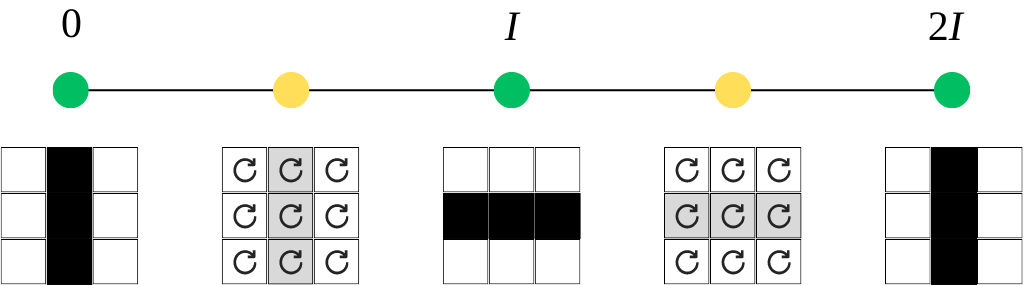
\includegraphics[width=0.8\textwidth]{imagenes/timeline}
  \caption{Ciclo de comunicación y actualización de una célula. En los puntos verdes, la célula comunica su estado a sus vecinas y se guarda el tablero. En los puntos intermedios amarillos, la célula actualiza su estado de acuerdo a las reglas del juego y al estado de sus vecinas.}\label{img:timeline}
\end{figure}

\begin{itemize}
  \item \textit{Comunicar}: la célula comunica su estado actual a sus vecinas y guarda en una variable interna el estado de su vecindario. Ocurre cada $I$ segundos comenzando por $t = 0$.
  \item \textit{Actualizar}: la célula actualiza su estado de acuerdo a dicha variable y a las reglas del juego. Ocurre cada $I$ segundos comenzando por $t = I/2$.
\end{itemize}

El fin de dividir el intervalo en dos subintervalos es separar las acciones de comunicar y actualizar para asegurar que cuando una célula calcule su nuevo estado todas sus vecinas le hayan comunicado el suyo.


\subsection{Formalización}


El DEVS que representa a una célula está definido como

\[ C = \langle X, Y, S, \dint, \dext, \lambda, ta \rangle \]

donde

\begin{itemize}
  \item $X = \N \times \{0,1\}$

    La entrada es un par $(id, s)$ que indica que el vecino con ese id nació ($s=1$) o murió ($s=0$).

  \item $Y = \big[ (\N \times \{0,1\}) \times \{0\} \big] \cup \{(0, 1)\}$

    La salida es de la forma $((id, s), 0)$ ó $(0, 1)$.

    Por el puerto 0 se emite el par $(id, s)$ con el id y estado actual de la célula.

    El puerto 1 se usa para descartar la salida cuando el estado de la célula no cambió.

  % S = (id, estado, vecinosVivos, vecindarioCambio, proximaAccion, sigma)
  \item $S = \N \times \{0, 1\} \times \N \times Bool \times \{Comunicar, Actualizar\} \times \R_0^+$

    El estado es una tupla $(id, s, vv, vc, pa, \sigma)$ donde

    \begin{itemize}
      \item $id \in \N$ es el identificador de la célula.
      \item $s \in \{0, 1\}$ es el estado actual de la célula.
      \item $vv \in \N$ es la cantidad de vecinos vivos.
      \item $vc \in Bool$ indica si el vecindario cambió en el último paso.
      \item $pa \in \{Comunicar, Actualizar\}$ indica la próxima acción a realizar.
      \item $\sigma \in \R_0^+$ es el tiempo restante para realizar la próxima acción.
    \end{itemize}

  \item $\dint(\estado) = \begin{cases}
      (id, s, vv, vc, Act, I/2) & pa = Com \\
      (id, s, vv, F, Act, I) & pa = Act \land \lnot vc \\
      (id, s, vv, F, Act, I) & pa = Act \land vc \land s = s' \\
      (id, s', vv, F, Com, I/2) & pa = Act \land vc \land s \neq s'
    \end{cases}$

    donde $s' = \text{calcularEstado}(s, vv)$.

    En este punto, $pa$ es la acción a realizar en el instante actual. Si ésta es \textit{Comunicar}, se reinicia el reloj interno y la próxima acción será \textit{Actualizar}.

    Si la acción es \textit{Actualizar} y el próximo estado es el mismo que el actual (casos 2 y 3) se evita la acción de \textit{Comunicar} estableciendo el reloj en $I$ y la $pa = Actualizar$.

    Por último, si el próximo estado es distinto del actual (caso 4), se establece la próxima acción en $Comunicar$ y se reinicia el reloj interno.

  \item $\dext(\estado, e, (id, x)) = (id, s, vv', T, pa, \sigma - e)$

    donde $vv' = \begin{cases}
      vv + 1 & x = 1 \\
      vv - 1 & x = 0
    \end{cases}$

  \item $\lambda(\estado) = \begin{cases}
      ((id, s), 0) & pa = Comunicar \\
      (0, 1) & pa = Actualizar
    \end{cases}$

    La célula produce una salida sólo en el caso de que la acción sea \textit{Comunicar}; si la acción es \textit{Actualizar} no ocurre una salida. Para simular esto, utilizamos el puerto 1 como descarte.

  \item $ta(\estado) = \sigma$
\end{itemize}

Consideramos a los parámetros $I \in \R^+$, que representa el tiempo entre estados del tablero, y $RS, RN \subseteq \N$ que representan a las reglas de supervivencia y nacimiento respectivamente. También utilizamos la función calcularEstado$()$ que es el próximo estado de una célula dado su estado actual y el número de vecinos vivos.

\[ \text{calcularEstado}(s, vv) = \begin{cases}
  1 & s = 1 \land vv \in RS \\
  1 & s = 0 \land vv \in RN \\
  0 & \text{en otro caso}
\end{cases}\]


\section{Implementación en PowerDEVS}


Una célula del tablero se implementa a través de un modelo DEVS atómico que incluye un parámetro para el id, una entrada y una salida, como se puede ver en la figura~\ref{img:celula}.

\begin{figure}[ht]
  \centering
  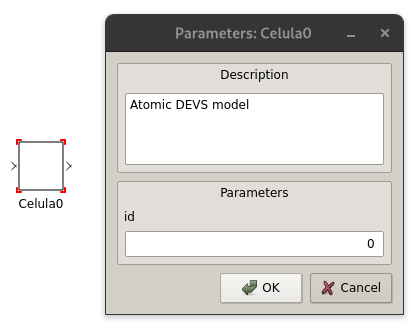
\includegraphics[width=0.5\textwidth]{imagenes/celula.png}
  \caption{Modelo atómico de una célula.}\label{img:celula}
\end{figure}

Una célula se comunica con sus vecinas a través de sus puertos de entrada y salida, como se observa en la figura~\ref{img:conexiones}. Por su puerto de entrada, a lo sumo 8 vecinas le comunican sus cambios de estado (fig.~\ref{img:coneciones_entrada}) y por su puerto de salida les comunica cuando cambia el suyo (fig.~\ref{img:coneciones_salida}).

\begin{figure}[ht]
  \centering
  \begin{subfigure}[b]{0.45\textwidth}
    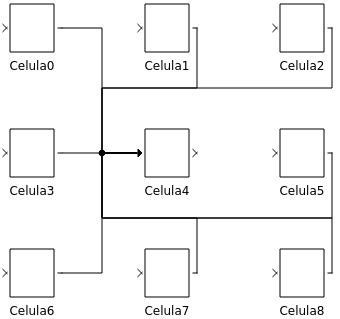
\includegraphics[width=\textwidth]{imagenes/entrada}
    \caption{Conexiones de entrada.}\label{img:coneciones_entrada}
  \end{subfigure}
  \hfill
  \begin{subfigure}[b]{0.45\textwidth}
    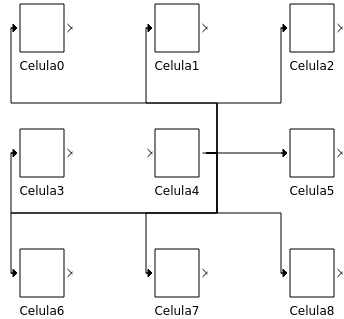
\includegraphics[width=\textwidth]{imagenes/salida}
    \caption{Conexiones de salida.}\label{img:coneciones_salida}
  \end{subfigure}
  \caption{Conexiones de una célula con sus vecinas.}\label{img:conexiones}
\end{figure}

En la figura~\ref{img:tablero} se observa un tablero completo de 4$\times$4 con las conexiones mencionadas anteriormente. Además, cada célula se comunica con un DEVs atómico `Escritor' que se encarga de escribir los resultados de una simulación en un archivo.

\begin{figure}[ht]
  \centering
  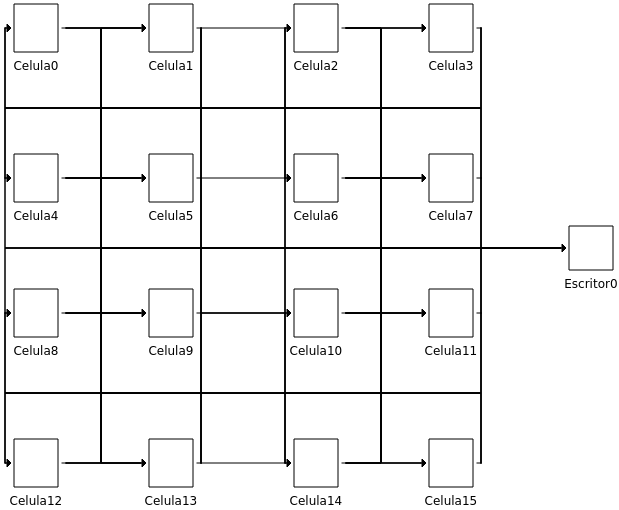
\includegraphics[width=0.75\textwidth]{imagenes/tablero.png}
  \caption{Tablero de 4$\times$4.}\label{img:tablero}
\end{figure}


\subsection{Flujo de evolución}

Cada célula, obtiene su estado inicial, las reglas de supervivencia y nacimiento, y el tiempo entre estados, a través de un archivo de configuración. De la misma manera, el Escritor obtiene el estado inicial del tablero y el tiempo entre estados del mismo archivo.

La simulación consta de dos etapas: una de \textit{Comunicación} y una de \textit{Actualización}. En la primera, cada célula comunica su estado a las vecinas y se escribe en un archivo de salida el estado actual del tablero. En la segunda, cada una actualiza su estado.

Para optimizar este proceso, se lleva una variable $vc \in Bool$ que indica si el vecindario cambió desde la última actualización. Si una célula está en la etapa de Actualización y $vc = F$ entonces no es necesario actualizar su estado, y por lo tanto tampoco es necesario comunicarlo a sus vecinas. Además, si el vecindario sí cambió ($vc = T$) pero el estado resultante es el mismo, tampoco es necesario comunicarlo. En estos casos, la célula no pasa por la etapa de Comunicación hasta que su estado cambie.

\end{document}
